\documentclass[11pt]{article}

\usepackage[a4paper,margin=1in]{geometry}
\usepackage[T1]{fontenc}
\usepackage[utf8]{inputenc}
\usepackage{lmodern}
\usepackage{microtype}
\usepackage{amsmath,amssymb}
\usepackage{graphicx}
\usepackage{booktabs}
\usepackage{array}
\usepackage{xcolor}
\usepackage[hidelinks]{hyperref}

\newcommand{\m}[1]{\texttt{#1}}
\newcommand{\dn}{\m{do\_nothing}}
\newcommand{\ro}{\m{retrain\_oracle}}
\newcommand{\roalt}{\m{retrain\_oracle\_alt}}
\newcommand{\cs}{\m{canary\_suppressor}}

\title{Proof of Forgetting? What Membership Tests Can and Cannot Certify in Federated Unlearning}
\author{Aaditya Tripathi\\[2pt]\normalsize Vellore Institute of Technology, Vellore, India}
\date{}

\begin{document}
\maketitle

\begin{abstract}
When a client asks a federated learning server to forget its data, the server
typically supports its claim with a membership-inference test showing that the
client can no longer be detected in the model. We ask what such tests can
certify, by running five verifiers against a server that did nothing at all,
against genuine retrains without the client, and against a dishonest server
that never unlearns but suppresses the client's backdoor canary. On CIFAR-10
(six seeds) and PathMNIST (three seeds) with ten non-IID clients, the
loss-threshold membership AUC most often reported for unlearning cannot tell
the server that did nothing from a genuine retrain on any run (AUC 0.48--0.55
for every model). Client-level LiRA, judged against ten retrains without the
client, separates them with one false alarm in 70 tests on genuine retrains,
but only when the client contributed enough data. Cutting a single client's
training data while holding the federation fixed shows that this size is the
cause: no client cut to 1000 samples or fewer was detected (0/6), while every
client with 3000 or more was (6/6). The threshold is not a constant: training
the federation longer (76--79\% instead of 61--67\% test accuracy) made a
1855-sample client detectable. Backdoor canaries are no safer: they flagged a
genuine retrain in 7 of 18 tests, and a server that reconstructs and erases the
trigger with Neural Cleanse passed the canary check on 2 of 9 runs and LiRA on
3 of 9. No single verifier caught the dishonest server on every run. Every
reported number is traceable to the run that produced it, and the code and
results are public.
\end{abstract}

\section{Introduction}

Data-protection rules such as the GDPR's right to erasure~\cite{gdpr} have
turned ``remove my data from your model'' into a request that model owners must
answer. Machine unlearning~\cite{cao2015,bourtoule2021} answers it by producing
a model that behaves as if the data had never been used, ideally the model one
would obtain by retraining without it. In federated learning
(FL)~\cite{mcmahan2017}, where the server never sees client data, the natural
unit of deletion is a whole client, and a growing set of methods remove a
client's contribution from a trained global
model~\cite{liu2021federaser,halimi2022}.

How is anyone to know that it worked? In practice, an unlearning method is
usually shown to work with a membership-inference attack (MIA): after
unlearning, the attack can no longer tell the forgotten data from data the
model never saw, so the data is declared forgotten. Two alternatives are
proposed for settings where the server is not trusted: the client can plant a
backdoor ``canary'' in its data and later check that the backdoor is
gone~\cite{sommer2022}, or the client can compare the model's behaviour on data
it trained with and data it held back. Each of these is a statistical test, and
a test is only as good as its behaviour on the cases where the answer is known.

This paper audits the tests rather than the unlearning methods. For every
verifier we ask two questions with known answers: does it catch a server that
did \emph{nothing} (\dn, which returns the original model), and does it pass a
genuine retrain without the client (\ro)? We then add a dishonest server that
never unlearns but tries to defeat the canary check. Our contributions:

\begin{itemize}
\item \textbf{The usual check is blind.} The loss-threshold membership AUC
cannot distinguish \dn{} from a retrain on any of 35 runs across two datasets
and two training lengths (Section~\ref{sec:v1}).
\item \textbf{Client-level LiRA works, within a limit we measure.} Judged
against ten retrains without the client, it detects \dn{} when the client is
large enough and raises one false alarm in 70 tests on genuine retrains
(Section~\ref{sec:lira}).
\item \textbf{The limit is the client's training size, and it moves with
training.} A controlled experiment that shrinks one client while holding the
rest of the federation fixed shows that the client's size causes the verdict;
auditing more samples does not help; training longer lowers the threshold
(Sections~\ref{sec:size} and~\ref{sec:longer}).
\item \textbf{Canaries can be suppressed, and they accuse honest servers.} A
server that never unlearns passed the canary check on 2 of 9 runs and LiRA on
3 of 9; the canary check flagged a genuine retrain in 7 of 18 tests
(Section~\ref{sec:dishonest}).
\item \textbf{Provenance.} Every number is written to an append-only ledger
with its run identifier, configuration hash, seed and code commit before it
enters a results file; the tables are generated from files that match the
ledger exactly.
\end{itemize}

\section{Background and related work}

\paragraph{Membership inference.} Shokri et al.~\cite{shokri2017} introduced
MIAs against trained models; Yeom et al.~\cite{yeom2018} showed that a
threshold on the per-example loss is already a strong baseline. Carlini et
al.~\cite{carlini2022} argued that average-case metrics such as AUC hide what
matters, the true-positive rate at very low false-positive rates, and proposed
LiRA: train reference (``shadow'') models with and without each example, fit a
Gaussian to the logit-scaled confidence under each hypothesis, and score a
target model by the likelihood ratio.

\paragraph{Verifying unlearning.} Sommer et al.~\cite{sommer2022} proposed
backdoor-based verification: a user poisons a fraction of its data with a
secret trigger and later tests whether the trigger still works. Thudi et
al.~\cite{thudi2022} showed that unlearning cannot be verified from the final
weights alone, since the same weights can be reached with or without a given
example, which motivates statistical rather than proof-based checks. Hayes et
al.~\cite{hayes2024} showed that commonly used MIA evaluations of unlearning
can give a false sense of privacy and that per-example reference models are
needed. In federated learning, Gao et al.~\cite{gao2022verifi} proposed a
verification framework in which the leaving client checks unlearning with
markers it controls.

\paragraph{Federated unlearning.} Methods that remove a client include
FedEraser~\cite{liu2021federaser}, which calibrates stored historical updates,
and projected gradient ascent by the departing client followed by a few rounds
of retraining~\cite{halimi2022}. Centralised methods such as
SCRUB~\cite{kurmanji2023} can be adapted. We use these methods only as
realistic unlearners; our object of study is the verifiers.

\paragraph{Backdoors and their removal.} BadNets~\cite{gu2017} showed that a
small trigger patch can implant a targeted backdoor. Neural
Cleanse~\cite{wang2019} reverse-engineers, for every class, the smallest
trigger that sends clean inputs to that class, flags the class whose trigger is
anomalously small, and removes the backdoor by fine-tuning. This is exactly the
tool a dishonest server would use against canary verification.

\section{Setup}

\subsection{Federation and data}

Ten clients receive a Dirichlet partition (concentration $\alpha=0.5$) of the
training set~\cite{hsu2019}. Each client splits its own data uniformly at
random into an \emph{in} half, which it trains with, and an \emph{out} half,
which it keeps private; the federation never sees any out half. We write
$n_f$ for the number of in-half (training) samples of the forgotten client;
client~0 is forgotten unless stated otherwise. The model is a ResNet-20~\cite{he2016}
of width 16 with GroupNorm~\cite{wu2018} instead of BatchNorm, so that a model
is a pure function of its parameters and no membership signal passes through
running statistics. FedAvg~\cite{mcmahan2017} runs 30 rounds (70 in
Section~\ref{sec:longer}) of 5 local epochs with all clients, SGD with learning
rate 0.05 (cosine schedule), momentum 0.9, weight decay $5\times10^{-4}$, batch
size 64, random crops and flips.

\textbf{CIFAR-10}~\cite{krizhevsky2009}: 50{,}000 training images; the official
test split is divided into a validation set (5000), a server-held auxiliary set
(1000) and the test set (4000). The federated model reaches 61--67\% test
accuracy at 30 rounds (the same code reaches 84.9\% trained centrally). On
seeds 42--47 the forgotten client holds $n_f =$ 3360, 2511, 1855, 1670, 4593 and
3667 training samples.

\textbf{PathMNIST}~\cite{yang2023medmnist,kather2019}: colorectal histology
patches, 9 classes, $28\times28$ colour. We draw 50{,}000 images from the
training split and pool the official validation and test splits as held-out
data, divided as above. The model reaches 80--82\%. On seeds 42--44 the
forgotten client holds 1900, 1111 and 3423 training samples.

\subsection{Unlearning methods}

All methods have the same interface and never read the forgotten client's out
half (a unit test enforces this).
\dn{} returns the original model: the negative control.
\ro{} retrains from scratch without the client with the same schedule and
per-client randomness; \roalt{} is a second retrain with different data order
and augmentation. Both are what an ideal unlearner would produce.
\m{finetune\_retain} continues FedAvg on the remaining clients for 5 rounds at
a small learning rate. \m{gradient\_ascent} lets the departing client maximise
its own loss with projected SGD inside an $\ell_2$ ball of 5\% of the model
norm, stops at the loss of a uniform guess, and then runs two recovery rounds
on the remaining clients~\cite{halimi2022}. \m{scrub} is a federated adaptation
of SCRUB~\cite{kurmanji2023}: the departing client runs a capped number of
max-steps against the original model, the remaining clients run min-steps, and
the server averages. \m{federaser\_lite} replays every original round with the
remaining clients, combining the direction of a short calibration update with
the stored per-layer size of the client's original update~\cite{liu2021federaser}.

\cs{} is dishonest. It never unlearns. Holding only the original model and
its own auxiliary data, it runs Neural Cleanse~\cite{wang2019} for every class,
picks the class with the most anomalous (smallest) reconstructed trigger, and
fine-tunes for 5 epochs on its auxiliary data with that trigger stamped on 20\%
of the images under their true labels. It does not know the client's trigger,
target class or data.

\subsection{Verifiers}

Each verifier answers ``is the forgotten client still in the model?'' with a
p-value or score. They differ in who can run them.

\textbf{V1, loss-threshold MIA (anyone).} The AUC of the score $-\ell(x)$ for
separating the client's in half (members) from its out half (non-members).
This is the check most commonly reported for unlearning; $0.5$ reads as
``forgotten''.

\textbf{V2, backdoor canary (client).} Before training, the client appends
triggered copies of 10\% of its training images, relabelled to a secret target
class, with a secret $4\times4$ pixel trigger at a secret position (as in
Athena~\cite{sommer2022}). To verify, it queries the model on the same
non-target test images with and without the trigger and applies an exact
one-sided McNemar test~\cite{mcnemar1947} to the discordant pairs: $b$ images
moved to the target by the trigger against $c$ moved away, under
$H_0\colon b\sim\mathrm{Binomial}(b+c,\tfrac12)$. A small p-value means the
backdoor, and so the client, is still in the model. V2 is used only in the
experiments with canaries (E2, E3).

\textbf{V3, client-level LiRA (auditor).} Following Carlini et
al.~\cite{carlini2022}, for each of the client's training samples we fit
Gaussians, with pooled variances, to the logit-scaled confidence of reference
models that did (IN) and did not (OUT) train with the client, and score the
target model by the log-likelihood ratio. The client's score is the mean over
its samples. The reference bank has 20 federations: ten retrains without the
client and ten full federations, all trained like the original. The null
distribution is the client's score on each of the ten OUT retrains, computed
leave-one-out so that no reference model is scored with its own statistics.
Because the null has only ten values, we use a Student-$t$ prediction test:
\[
t=\frac{s-\bar s_0}{\hat\sigma_0\sqrt{1+1/10}}\quad\text{with 9 degrees of freedom},
\]
and report $z=(s-\bar s_0)/\hat\sigma_0$ alongside $p$. At $\alpha=0.05$ a
target is ``detected'' when $t>1.83$.

\textbf{V4, distance to the oracle (server).} Weight-space and prediction-space
distance to \ro, read against the distance between the two retrains. In our
runs two retrains differ about as much as the original differs from either, so
V4 is not informative and we do not discuss it further.

\textbf{V5, in/out permutation test (client).} The client compares the model's
logit-scaled confidence on its in half and its out half with an exact
permutation test (10{,}000 permutations): a model that still contains the
client fits the in half better. Only the client's own data and black-box access
to the model are needed.

\subsection{Experiments and statistics}

\textbf{E0} applies every method and scores every model with V1, V3, V4 and V5.
\textbf{E2} plants canaries, follows gradient ascent (no early stop, no
recovery) and scores V2, V3 and V5 every four steps. \textbf{E3} plants
canaries and adds \cs. \textbf{E4} subsamples the client's halves to fixed
sizes and measures V5's power. \textbf{E5} measures the raw attack strength of
loss and LiRA on the reference bank. Three further sets of E0 runs vary one
factor: \emph{client swaps} forget a different client in an existing federation
(seed 42 client 5, seed 45 client 8); \emph{controlled cuts} train the forgotten
client with a random subset of 500, 1000, 2000 or 3000 of its samples (its out
half cut in proportion) while every other client and all randomness stay
fixed (seeds 42, 46, 47); and \emph{longer training} uses 70 rounds (seeds
42--44). E0, E2, E3 and E5 ran on six CIFAR-10 seeds (42--47) and E0, E2 and E3
on three PathMNIST seeds (42--44); E4 ran on the six CIFAR-10 seeds.

All tests are one-sided at $\alpha=0.05$; we report p-values rather than
correcting for multiplicity, and count detections across runs. Every random
draw is keyed by (seed, purpose, round, client) and training is bitwise
deterministic on a fixed device.

\paragraph{Design changes after seeing data.} Four choices were revised after
the first seed (42) and before any other seed ran: five local epochs instead of
two (two gave about 43\% accuracy and almost no memorisation); V5 on
logit-scaled confidence instead of loss (mean loss is heavy-tailed and flagged
a retrain whose accuracy on both halves was identical); V3's null made of
retrains without the client, with the prediction test (a null of smaller
balanced federations scored a second retrain at $z=4.3$); and capped SCRUB
max-steps and every-round FedEraser replay (otherwise both collapsed). The
70-round setting was chosen from a tuning run on seed 42 (90 rounds reached
79.4\% but did not fit the 12-hour compute sessions we used). Every later run is
therefore a test of these choices.

\section{Results}

\subsection{The standard check cannot tell ``did nothing'' from ``retrained''}
\label{sec:v1}

\begin{figure}[t]
\centering
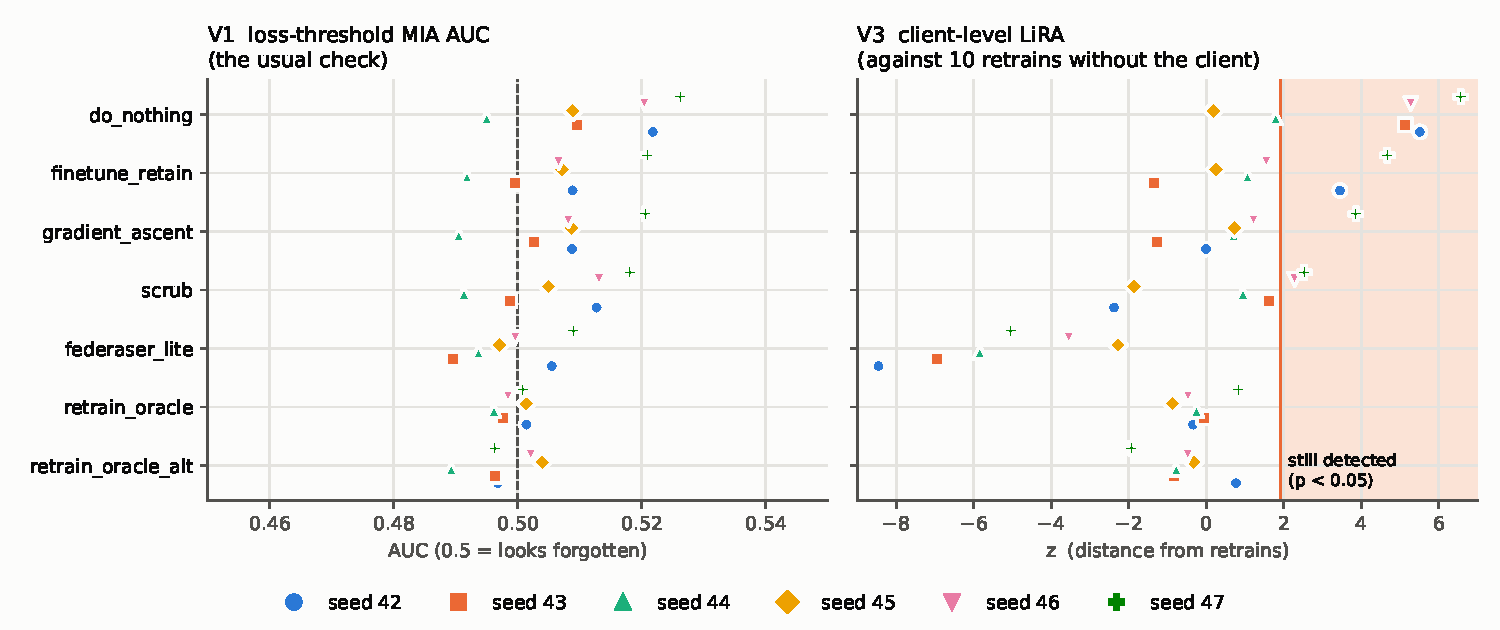
\includegraphics[width=\linewidth]{figures/verifiers.pdf}
\caption{Every model on the six CIFAR-10 seeds. Left: V1, the loss-threshold
membership AUC, is between 0.489 and 0.526 for every model, including the
server that did nothing and both genuine retrains. Right: V3, client-level
LiRA, places \dn{} far above the retrains on four seeds; the shaded region is
detection at $p<0.05$.}
\label{fig:verifiers}
\end{figure}

V1 reads between 0.489 and 0.526 for all seven models on all six CIFAR-10 seeds
(Figure~\ref{fig:verifiers}, left): for \dn{} 0.522, 0.510, 0.495, 0.509, 0.520
and 0.526; for the two retrains 0.489--0.504. The same holds on PathMNIST
(0.507--0.517 for \dn) and for the longer-trained models (0.523--0.552).
Across all 35 E0 and E3 runs, every model lies between 0.476 and 0.552. A
server could return the original model and report ``AUC $\approx 0.5$, client
forgotten''. This is hypothesis H1, fixed before any run, and it holds on every
run.

Attack strength explains why. In E5, the per-sample loss attack reaches AUC
0.515--0.662 on CIFAR-10 at the sample level (LiRA 0.495--0.797), and at most
4.3\% true positives at 1\% false positives. Per-sample membership signal in
these models is weak; it is the aggregate over a client that carries
information, which V1's average does not exploit and V3 does.

\subsection{LiRA separates them, and almost never accuses a retrain}
\label{sec:lira}

\begin{table}[t]
\centering
\caption{V3 on the main CIFAR-10 runs. $n_f$: training samples of the forgotten
client. Detected at $\alpha=0.05$ in bold.}
\label{tab:v3}
\small
\begin{tabular}{lcccccc}
\toprule
 & seed 42 & seed 43 & seed 44 & seed 45 & seed 46 & seed 47\\
\midrule
$n_f$ & 3360 & 2511 & 1855 & 1670 & 4593 & 3667\\
\dn{} $z$ & \textbf{5.5} & \textbf{5.1} & 1.8 & 0.2 & \textbf{5.3} & \textbf{6.6}\\
\dn{} $p$ & \textbf{0.0003} & \textbf{0.0004} & 0.061 & 0.43 & \textbf{0.0004} & $\mathbf{<0.0001}$\\
\ro{} $p$ & 0.62 & 0.52 & 0.59 & 0.79 & 0.67 & 0.23\\
\roalt{} $p$ & 0.24 & 0.78 & 0.76 & 0.62 & 0.67 & 0.95\\
\bottomrule
\end{tabular}
\end{table}

V3 detects \dn{} clearly on four CIFAR-10 seeds, marginally on seed 44 and not
at all on seed 45 (Table~\ref{tab:v3}). Across every E0 and E3 run (both
datasets, all client sizes, both training lengths) the two retrains were tested
70 times and V3 flagged one (PathMNIST seed 44 in E3, $p=0.017$): a 1.4\% false
alarm rate, below the nominal 5\%.

Of the honest unlearning methods, those that keep their accuracy are often
still detected: \m{finetune\_retain} on seeds 42 and 47 ($p=0.005$, 0.0008),
\m{gradient\_ascent} on seed 47 ($p=0.003$), \m{scrub} on seeds 46 and 47
($p=0.03$, 0.02). \m{federaser\_lite} is never detected but loses 11--22 points
of accuracy; a model that ``forgets'' by getting worse at everything is not the
retrain.

\subsection{What decides LiRA's verdict is the client's training size}
\label{sec:size}

\begin{figure}[t]
\centering
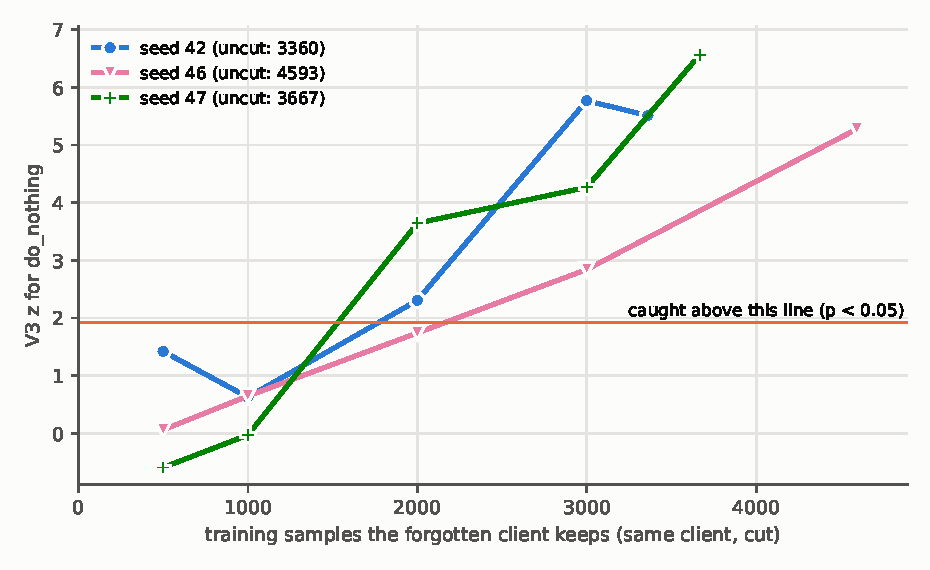
\includegraphics[width=0.8\linewidth]{figures/controlled_size.pdf}
\caption{Controlled client size. The same forgotten client is trained with
500--3000 of its samples while the rest of the federation is unchanged; the
rightmost point of each line is the uncut client. V3 $z$ for \dn; above the
line is detection at $p<0.05$.}
\label{fig:controlled}
\end{figure}

\paragraph{Auditing more samples does not help.} Rerunning V3 on random
subsets of $m$ of the client's samples (200 subsets per size, no retraining),
the median $z$ for \dn{} levels off by $m=250$--500 on every seed: for example
3.3, 4.8, 5.2, 5.5 at $m=$ 50, 250, 500, 1500 on seed 42, and 1.1, 1.6, 1.8, 1.8
on seed 44 (Figure~\ref{fig:audit} in the appendix). Retrains were flagged in at
most 6.5\% of subsets at any $m$ and in none once $m\ge1000$. A weak verdict
cannot be rescued by auditing more of the client's data.

\paragraph{Shrinking the client changes the verdict.} The controlled cuts
(Table~\ref{tab:cuts}, Figure~\ref{fig:controlled}) hold the seed, the other
nine clients and all randomness fixed and change only how much of the forgotten
client's data is used. No client cut to 1000 samples or fewer was detected
(0/6); at 2000, two of three were; at 3000 or more, all were (6/6). The retrains
were never flagged in these runs. Cutting a large client also removes data from
the federation: seed 46's accuracy fell from 61\% to 54--57\%; the other two
seeds lost about 3 points or less.

\begin{table}[t]
\centering
\caption{V3 $z$ for \dn{} when the forgotten client keeps only part of its data.
Detected at $\alpha=0.05$ in bold.}
\label{tab:cuts}
\small
\begin{tabular}{lccccc}
\toprule
client keeps & 500 & 1000 & 2000 & 3000 & all\\
\midrule
seed 42 (all $=$ 3360) & 1.4 & 0.6 & \textbf{2.3} & \textbf{5.8} & \textbf{5.5}\\
seed 46 (all $=$ 4593) & 0.1 & 0.7 & 1.7 & \textbf{2.8} & \textbf{5.3}\\
seed 47 (all $=$ 3667) & $-0.6$ & 0.0 & \textbf{3.6} & \textbf{4.3} & \textbf{6.6}\\
\bottomrule
\end{tabular}
\end{table}

\paragraph{Natural clients agree.} Across the eight main CIFAR-10 runs (six
seeds and two client swaps), every forgotten client with at least 2511 training
samples was detected (5/5, $z=4.4$--6.6) and every client with at most 1855 was
not (0/3, $z=0.2$--1.9) (Figure~\ref{fig:clientsize} in the appendix). The swaps
show it is the client, not the federation: in the seed-45 federation, client 0
(1670 samples) gives $z=0.2$ and client 8 (3345) gives $z=4.4$; in seed 42,
client 0 (3360) gives 5.5 and client 5 (1515) gives 1.9. On PathMNIST only the
large client was detected (3423 samples, $z=3.3$, $p=0.006$), not the small ones
(1900: $z=-2.5$; 1111: $z=0.5$).

\subsection{A better-trained model is easier to audit}
\label{sec:longer}

\begin{table}[t]
\centering
\caption{The same federations trained for 30 and 70 rounds. Detected at
$\alpha=0.05$ in bold.}
\label{tab:longer}
\small
\begin{tabular}{lccc}
\toprule
 & seed 42 & seed 43 & seed 44\\
\midrule
$n_f$ & 3360 & 2511 & 1855\\
test accuracy, 30 $\to$ 70 rounds & 64.9 $\to$ 77.5\% & 63.9 $\to$ 76.3\% & 67.1 $\to$ 78.7\%\\
V3 $z$ for \dn, 30 rounds & \textbf{5.5} & \textbf{5.1} & 1.8\\
V3 $z$ for \dn, 70 rounds & \textbf{8.6} & \textbf{6.5} & \textbf{3.2}\\
V5 $p$ for \dn, 30 rounds & \textbf{0.0002} & 0.10 & 0.59\\
V5 $p$ for \dn, 70 rounds & \textbf{0.0001} & \textbf{0.0001} & \textbf{0.0006}\\
\bottomrule
\end{tabular}
\end{table}

The main runs are undertrained relative to the architecture: in a tuning run,
90 rounds reached 79.4\% while doubling the width did not help (65.3\% at 30
rounds). Rerunning three seeds at 70 rounds (Table~\ref{tab:longer}) raised
V3's evidence on every seed, and seed 44's 1855-sample client, undetectable at
30 rounds, was detected at 70 by both V3 ($p=0.007$) and V5. Longer training
memorises more: in tuning, the gap between the client's training accuracy and
test accuracy grew from 4.5 points at 30 rounds to 12 at 90. No retrain was
flagged (V3 $p\ge0.41$, V5 $p\ge0.11$). The size threshold of
Section~\ref{sec:size} is therefore a property of the setup, and part of what
looks like ``small clients cannot be audited'' is an undertrained model. V1
stays blind (0.523--0.552).

\subsection{A dishonest server, and canaries that accuse honest servers}
\label{sec:dishonest}

\begin{table}[t]
\centering
\caption{E3: the dishonest \cs{} against each verifier. NC: whether Neural
Cleanse picked the client's secret target class. ``Fooled'' marks a verifier
that no longer detects a server that forgot nothing ($p>0.05$).}
\label{tab:e3}
\small
\begin{tabular}{lcccc}
\toprule
 & NC class & V2 (canary) $p$ & V3 (LiRA) $p$ & V5 (own data) $p$\\
\midrule
CIFAR-10 seed 42 & no & $<0.0001$ & $<0.0001$ & 0.048\\
CIFAR-10 seed 43 & no & 0.0003 & $<0.0001$ & 0.27\\
CIFAR-10 seed 44 & no & \textbf{0.97, fooled} & 0.021 & 0.30\\
CIFAR-10 seed 45 & no & $<0.0001$ & 0.018 & 0.14\\
CIFAR-10 seed 46 & \textbf{yes} & \textbf{1.00, fooled} & \textbf{0.15, fooled} & 0.0003\\
CIFAR-10 seed 47 & no & 0.032 & $<0.0001$ & 0.013\\
PathMNIST seed 42 & no & $<0.0001$ & \textbf{0.59, fooled} & 0.15\\
PathMNIST seed 43 & no & $<0.0001$ & \textbf{0.16, fooled} & 0.37\\
PathMNIST seed 44 & no & $<0.0001$ & $<0.0001$ & 0.038\\
\bottomrule
\end{tabular}
\end{table}

\cs{} never unlearns, so every verifier should detect it. Table~\ref{tab:e3}
shows that each was fooled at least once and none caught it on every run. The
canary check certified it on two CIFAR-10 seeds: on seed 44 the canary was weak
to begin with (trigger success 9\% on \dn, against 90\% on seed 42), and on
seed 46 Neural Cleanse found the client's actual target class, after which the
suppressor got past LiRA too, at a cost of 7 points of accuracy. On PathMNIST
it got past LiRA on two of three seeds without finding the class, while keeping
its accuracy (83.6\% and 81.7\%, against 81.4\% and 81.3\% for \dn). This
supports H3: the canary can be removed without knowledge of the trigger and
without forgetting.

The canary check also fires on honest servers. It flagged a genuine retrain in
3 of 12 tests on CIFAR-10 and 4 of 6 on PathMNIST (7 of 18 in all). On PathMNIST
it therefore rejects the honest server about as often as the dishonest one; a
canary that fires is not evidence that the server failed to forget.

\subsection{Do canaries disappear first?}
\label{sec:e2}

\begin{figure}[t]
\centering
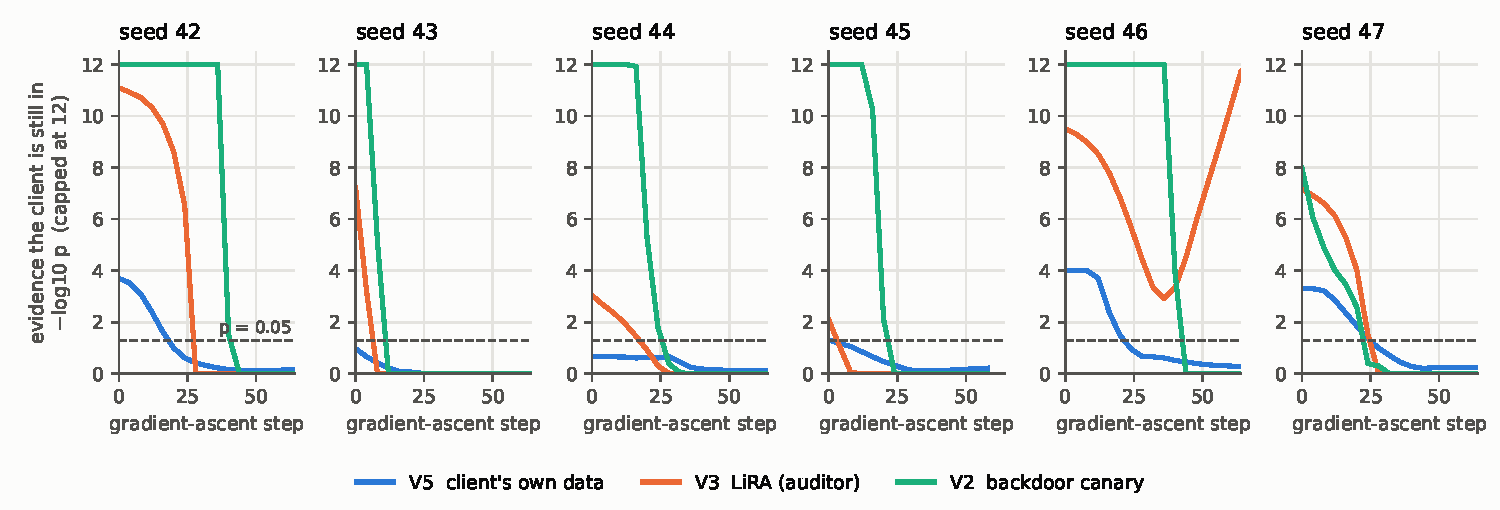
\includegraphics[width=\linewidth]{figures/gradient_ascent.pdf}
\caption{Evidence that the client is still in the model ($-\log_{10}p$, capped
at 12) along gradient ascent, CIFAR-10. The dashed line is $p=0.05$.}
\label{fig:ascent}
\end{figure}

H2 predicted that gradient ascent removes the sharply memorised canary before
the client's ordinary influence. Following ascent step by step
(Figure~\ref{fig:ascent}), the canary was usually the \emph{last} signal to go:
on CIFAR-10 seeds 42--45 and PathMNIST seed 44, V2 still detected the client
after V3 and V5 had stopped. On CIFAR-10 seed 46 and PathMNIST seed 43, LiRA
outlasted the canary but only into a model near chance accuracy, where V3's
score means little. On CIFAR-10 seed 47 and PathMNIST seed 42 the canary went
first, as H2 predicted, while the model was still accurate (58\% and 72\%). H2
holds on 2 of 9 runs; the canary going last is the usual order but not a rule.

\subsection{The client's own test needs a large client or a well-trained model}
\label{sec:v5}

V5 needs only the client's data. On the main CIFAR-10 runs it detected \dn{}
on seeds 42, 46 and 47 ($p=0.0002$, 0.0002, $<0.0001$) and not on 43, 44 or 45
(0.10, 0.59, 0.10). Including the swaps, it detected every forgotten client
with at least 3345 training samples (4/4) and none with 2511 or fewer (0/4). In
the controlled cuts it detected every client cut to 2000 or more (6/6) and one
of six cut to 1000 or fewer; it detected nothing on PathMNIST (0/3) and all
three clients at 70 rounds. It flagged a genuine retrain once in 52 E0 tests
(PathMNIST seed 42, $p=0.011$). In E4, which fixes the client's halves at
100--2500 samples each, V5 detected \dn{} at some sizes on seeds 42, 45 and 47
and at none on 43, 44 and 46, and flagged the retrain in 2 of 28 tests. H4, a
minimum client size for V5, is supported, but the minimum also depends on the
federation and on how well the model is trained.

\section{Discussion}

\paragraph{What to report.} An unlearning claim backed by a loss-threshold MIA
AUC near 0.5 says nothing in our setting: the same number is produced by a
server that did nothing. A verifier should be reported with its result on
\dn{} and on a genuine retrain, which costs one extra model and one retrain.

\paragraph{Who can verify.} The verifier that worked best, client-level LiRA
against retrains without the client, needs those retrains: only the server or
an auditor with comparable compute can produce them. The checks a client can
run alone are weaker. V5 works only for large clients or well-trained models,
and canaries must be planted in advance, can be suppressed, and raise false
alarms. A practical protocol therefore combines checks: no single one caught
the dishonest server on every run, but on every run at least one of V2, V3 and
V5 did (though on PathMNIST V2 fires on genuine retrains as well).

\paragraph{Small clients.} Below roughly 2000 training samples in our 30-round
setting, no verifier could tell a server that did nothing from one that
retrained. A client that contributed little is, in this sense, already hard to
distinguish from one that was never there, and its deletion cannot be
verified by these means. The threshold falls as models memorise more, so it
should be measured for each deployment rather than assumed.

\section{Limitations}

We use one architecture (ResNet-20), one degree of non-IID partition
($\alpha=0.5$), ten clients with full participation, and two image datasets.
Most results are at 61--67\% accuracy on CIFAR-10; the 70-round runs show that
the main conclusions hold at 76--79\% but cover only E0. PathMNIST has three
seeds. The client-size evidence rests on eight natural clients and twelve
controlled cuts on CIFAR-10 and three clients on PathMNIST; the thresholds we
report depend on the setup. The dishonest server is a single attacker, an
adaptive Neural Cleanse variant; stronger attackers could do better against
V3 and V5. V3 assumes the model under test resembles its reference models; for
a model that has collapsed to chance accuracy its score is extreme and
uninformative. V5 and V3's prediction test were chosen after seeing seed 42,
so seed 42 is not evidence for them; every later run is.

\section{Conclusion}

Membership-inference verification of federated unlearning can be done, but not
with the test most often used, not for every client, and not by the client
alone. Client-level LiRA against retrains without the client separates a
server that did nothing from one that retrained, with few false alarms, as long
as the client contributed enough data; a controlled experiment shows that this
size is the cause, and longer training lowers it. Backdoor canaries are
neither safe from a dishonest server nor safe to trust when they fire. We
release the code, every result file and the ledger that ties each number in
this paper to the run that produced it.

\section*{Code and data availability}

Code, configurations, result files and the results ledger:
\url{https://github.com/aaditripi18/Proof-of-Forgetting}. The repository's
\texttt{docs/RESULTS.md} lists every number with its run identifier,
configuration hash and code commit, and is generated from result files that a
test checks against the ledger.

\section*{Acknowledgements}

The experiments ran on free Kaggle GPUs. The author used Claude (Anthropic), an
AI assistant, for help with writing code, running experiments and drafting the
text; the author reviewed all of the content and takes full responsibility for
it.

\begin{thebibliography}{99}
\small

\bibitem{bourtoule2021}
L.~Bourtoule, V.~Chandrasekaran, C.~A. Choquette-Choo, H.~Jia, A.~Travers,
B.~Zhang, D.~Lie, and N.~Papernot.
\newblock Machine unlearning.
\newblock In \emph{IEEE Symposium on Security and Privacy (S\&P)}, 2021.

\bibitem{cao2015}
Y.~Cao and J.~Yang.
\newblock Towards making systems forget with machine unlearning.
\newblock In \emph{IEEE Symposium on Security and Privacy (S\&P)}, 2015.

\bibitem{carlini2022}
N.~Carlini, S.~Chien, M.~Nasr, S.~Song, A.~Terzis, and F.~Tram\`er.
\newblock Membership inference attacks from first principles.
\newblock In \emph{IEEE Symposium on Security and Privacy (S\&P)}, 2022.

\bibitem{gao2022verifi}
X.~Gao, X.~Ma, J.~Wang, Y.~Sun, B.~Li, S.~Ji, P.~Cheng, and J.~Chen.
\newblock {VeriFi}: Towards verifiable federated unlearning.
\newblock \emph{arXiv preprint arXiv:2205.12709}, 2022.

\bibitem{gdpr}
European Parliament and Council of the European Union.
\newblock Regulation ({EU}) 2016/679 (General Data Protection Regulation),
Article~17: Right to erasure.
\newblock \emph{Official Journal of the European Union}, L 119, 2016.

\bibitem{gu2017}
T.~Gu, B.~Dolan-Gavitt, and S.~Garg.
\newblock {BadNets}: Identifying vulnerabilities in the machine learning model
supply chain.
\newblock \emph{arXiv preprint arXiv:1708.06733}, 2017.

\bibitem{halimi2022}
A.~Halimi, S.~Kadhe, A.~Rawat, and N.~Baracaldo.
\newblock Federated unlearning: How to efficiently erase a client in {FL}?
\newblock \emph{arXiv preprint arXiv:2207.05521}, 2022.

\bibitem{hayes2024}
J.~Hayes, I.~Shumailov, E.~Triantafillou, A.~Khalifa, and N.~Papernot.
\newblock Inexact unlearning needs more careful evaluations to avoid a false
sense of privacy.
\newblock \emph{arXiv preprint arXiv:2403.01218}, 2024.

\bibitem{he2016}
K.~He, X.~Zhang, S.~Ren, and J.~Sun.
\newblock Deep residual learning for image recognition.
\newblock In \emph{IEEE Conference on Computer Vision and Pattern Recognition
(CVPR)}, 2016.

\bibitem{hsu2019}
T.-M.~H. Hsu, H.~Qi, and M.~Brown.
\newblock Measuring the effects of non-identical data distribution for
federated visual classification.
\newblock \emph{arXiv preprint arXiv:1909.06335}, 2019.

\bibitem{kather2019}
J.~N. Kather, J.~Krisam, P.~Charoentong, T.~Luedde, E.~Herpel, C.-A. Weis,
T.~Gaiser, A.~Marx, N.~A. Valous, D.~Ferber, L.~Jansen, C.~C. Reyes-Aldasoro,
I.~Z\"ornig, D.~J\"ager, H.~Brenner, J.~Chang-Claude, M.~Hoffmeister,
N.~Halama.
\newblock Predicting survival from colorectal cancer histology slides using
deep learning: A retrospective multicenter study.
\newblock \emph{PLoS Medicine}, 16(1):e1002730, 2019.

\bibitem{krizhevsky2009}
A.~Krizhevsky.
\newblock Learning multiple layers of features from tiny images.
\newblock Technical report, University of Toronto, 2009.

\bibitem{kurmanji2023}
M.~Kurmanji, P.~Triantafillou, J.~Hayes, and E.~Triantafillou.
\newblock Towards unbounded machine unlearning.
\newblock In \emph{Advances in Neural Information Processing Systems
(NeurIPS)}, 2023.

\bibitem{liu2021federaser}
G.~Liu, X.~Ma, Y.~Yang, C.~Wang, and J.~Liu.
\newblock {FedEraser}: Enabling efficient client-level data removal from
federated learning models.
\newblock In \emph{IEEE/ACM International Symposium on Quality of Service
(IWQoS)}, 2021.

\bibitem{mcmahan2017}
B.~McMahan, E.~Moore, D.~Ramage, S.~Hampson, and B.~A. y~Arcas.
\newblock Communication-efficient learning of deep networks from decentralized
data.
\newblock In \emph{International Conference on Artificial Intelligence and
Statistics (AISTATS)}, 2017.

\bibitem{mcnemar1947}
Q.~McNemar.
\newblock Note on the sampling error of the difference between correlated
proportions or percentages.
\newblock \emph{Psychometrika}, 12(2):153--157, 1947.

\bibitem{shokri2017}
R.~Shokri, M.~Stronati, C.~Song, and V.~Shmatikov.
\newblock Membership inference attacks against machine learning models.
\newblock In \emph{IEEE Symposium on Security and Privacy (S\&P)}, 2017.

\bibitem{sommer2022}
D.~M. Sommer, L.~Song, S.~Wagh, and P.~Mittal.
\newblock Athena: Probabilistic verification of machine unlearning.
\newblock \emph{Proceedings on Privacy Enhancing Technologies (PoPETs)},
2022(3), 2022.

\bibitem{thudi2022}
A.~Thudi, H.~Jia, I.~Shumailov, and N.~Papernot.
\newblock On the necessity of auditable algorithmic definitions for machine
unlearning.
\newblock In \emph{USENIX Security Symposium}, 2022.

\bibitem{wang2019}
B.~Wang, Y.~Yao, S.~Shan, H.~Li, B.~Viswanath, H.~Zheng, and B.~Y. Zhao.
\newblock Neural {C}leanse: Identifying and mitigating backdoor attacks in
neural networks.
\newblock In \emph{IEEE Symposium on Security and Privacy (S\&P)}, 2019.

\bibitem{wu2018}
Y.~Wu and K.~He.
\newblock Group normalization.
\newblock In \emph{European Conference on Computer Vision (ECCV)}, 2018.

\bibitem{yang2023medmnist}
J.~Yang, R.~Shi, D.~Wei, Z.~Liu, L.~Zhao, B.~Ke, H.~Pfister, and B.~Ni.
\newblock {MedMNIST} v2 -- a large-scale lightweight benchmark for 2{D} and
3{D} biomedical image classification.
\newblock \emph{Scientific Data}, 10:41, 2023.

\bibitem{yeom2018}
S.~Yeom, I.~Giacomelli, M.~Fredrikson, and S.~Jha.
\newblock Privacy risk in machine learning: Analyzing the connection to
overfitting.
\newblock In \emph{IEEE Computer Security Foundations Symposium (CSF)}, 2018.

\end{thebibliography}

\appendix
\section{Additional figures}

\begin{figure}[h]
\centering
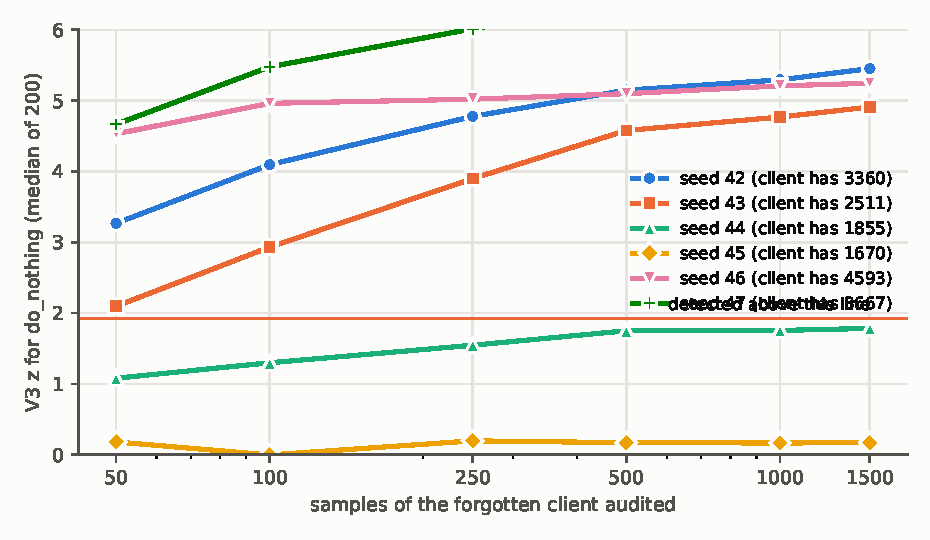
\includegraphics[width=0.8\linewidth]{figures/audit_size.pdf}
\caption{V3 $z$ for \dn{} (median over 200 random subsets) against the number
of the client's samples audited, without retraining. The evidence levels off by
250--500 samples on every seed.}
\label{fig:audit}
\end{figure}

\begin{figure}[h]
\centering
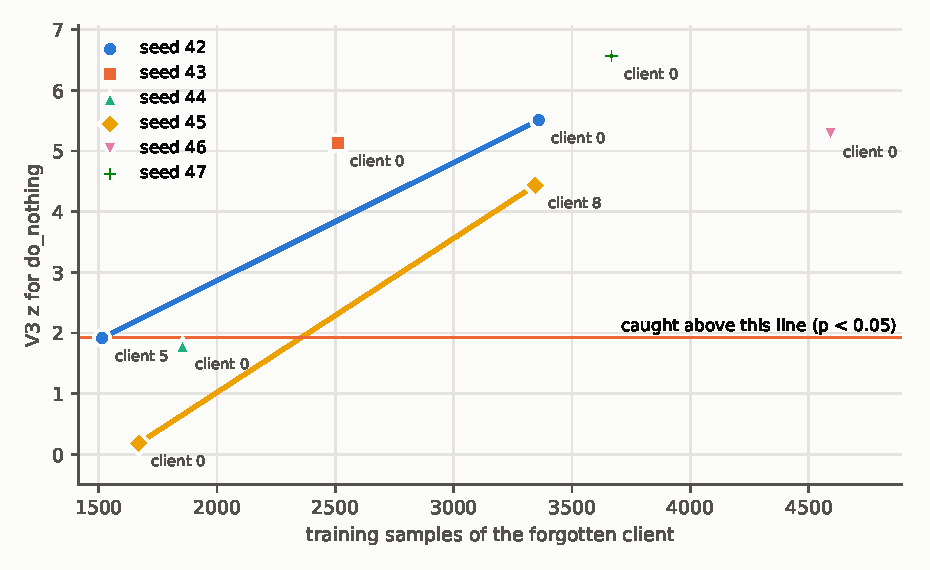
\includegraphics[width=0.8\linewidth]{figures/client_size.pdf}
\caption{V3 $z$ for \dn{} against the forgotten client's training size, for
the six seeds and two client swaps (joined lines: two clients of the same
federation).}
\label{fig:clientsize}
\end{figure}

\end{document}
